\documentclass{article}
\usepackage[margin=1in]{geometry}
\usepackage{mathtools, amsfonts, amsthm, graphicx, listings, xcolor}

\definecolor{codegreen}{rgb}{0,0.6,0}
\definecolor{codegray}{rgb}{0.5,0.5,0.5}
\definecolor{codepurple}{rgb}{0.58,0,0.82}
\definecolor{backcolour}{rgb}{0.95,0.95,0.92}

\lstdefinestyle{mystyle}{
    backgroundcolor=\color{backcolour},   
    commentstyle=\color{codegreen},
    keywordstyle=\color{magenta},
    numberstyle=\tiny\color{codegray},
    stringstyle=\color{codepurple},
    basicstyle=\ttfamily\footnotesize,
    breakatwhitespace=false,         
    breaklines=true,                 
    captionpos=b,                    
    keepspaces=true,                 
    numbers=left,                    
    numbersep=5pt,                  
    showspaces=false,                
    showstringspaces=false,
    showtabs=false,                  
    tabsize=2
}

\lstset{style=mystyle}

\title{HW01 Graphs and Social Networks}
\author{Sam Ly}


\begin{document}
\maketitle

\section*{Q1 (5 pts)}

\begin{enumerate}
    \item {
        Draw the graph.
        \begin{figure}[htbp]
            \centering
            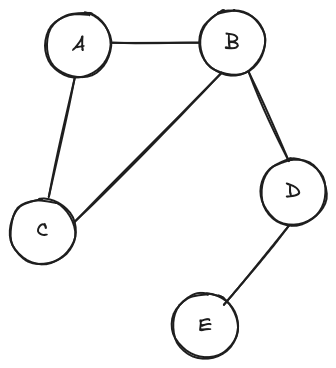
\includegraphics[width=0.4\textwidth]{graph.png}
        \end{figure}
    }

    \item {
        Compute the degree of each node.

        \[ \text{deg}(A) = 2 \]
        \[ \text{deg}(B) = 3 \]
        \[ \text{deg}(C) = 2 \]
        \[ \text{deg}(D) = 2 \]
        \[ \text{deg}(E) = 1 \]
    }

    \item {
        Verify the \textbf{Handshake Theorem}.

        \[\sum_{v \in V}{\text{deg}(v)} = 2 |E| \]

        \[2+3+2+2+1 = 10 = 2 |E| \]
    }

    \item {
        Explain briefly why this must always hold for undirected graphs.

        This must always hold true for undirected graphs because each edge
        always connects two nodes. This means those two nodes increase their
        degree by one when connected by one edge. By extension, each edge 
        increases the sum of all node degrees. 

        Therefore, the sum of all degrees of nodes is equal to two times the 
        number of edges.
    }
\end{enumerate}

\section*{Q2 (5 pts)}

\begin{enumerate}
    \item {
        Write down the \textbf{degree distribution}: how many nodes have degree 1, 2, 3, etc.

        \begin{table}[htbp]
            \centering
            \begin{tabular}{cc}
                Degree & No. of Nodes \\
                1 & 1 \\
                2 & 3 \\
                3 & 1 \\

            \end{tabular}
        \end{table}
    }

    \item {
        Write a short \textbf{Python snippet} that:
        \begin{itemize}
            \item Stores the graph as a dictionary of neighbors.
            \item Loops over nodes to compute degrees.
            \item Prints the degree distribution.
        \end{itemize}

        \lstinputlisting[language=Python, firstline=1, lastline=19]{./code/main.py}        
    }

    \item {
        Make a \textbf{bar chart} of the distribution (x = degree, y = count). Label axes and add a title.
        \begin{figure}[htbp]
            \centering
            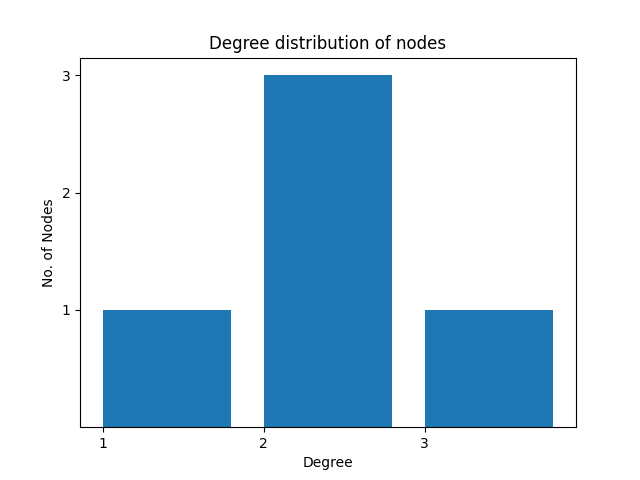
\includegraphics[width=0.5\textwidth]{bar.png}
        \end{figure} 
    }
\end{enumerate}

\section*{Q3 (5 pts)}

\begin{enumerate}
    \item {
        List its connected components.

        All nodes are in one connected component, thus the only connected
        component is \(\{A, B, C, D, E\}\)
    }

    \item {
        Suppose the edge \textbf{D–E} is removed.
        How many components now? Which nodes are in each?

        \begin{figure}[htbp]
            \centering
            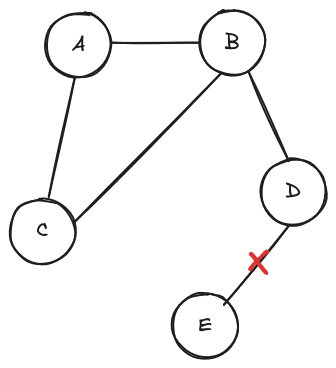
\includegraphics[width=0.4\textwidth]{graph_no_DE.png}
        \end{figure}

        There are now 2 connected components:
        \begin{itemize}
            \item \(\{A, B, C, D\}\), 4 nodes.
            \item \(\{E\}\), 1 node.
        \end{itemize}
    }

    \item {
        Is \textbf{D-E} a \textbf{bridge} (an edge whose removal increases the 
        number of components)? Justify in one sentence.

        \textbf{D-E} is a bridge because it is the only edge that connects node 
        \textbf{E} to the rest of the graph, thus removing it makes node \textbf{E}
        a new component.
    }
\end{enumerate}

\section*{Q4 (5 pts)}

Consider this undirected graph:
\\Nodes = \(\{P, Q, R, S, T\}\)
\\Edges = \( \{ P-Q, Q-R, Q-S, R-T \} \)

\begin{figure}[htbp]
    \centering
    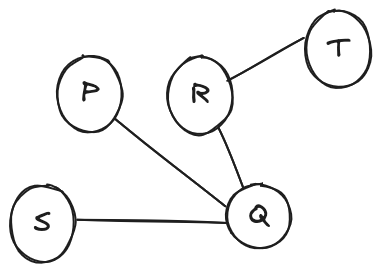
\includegraphics[width=0.5\textwidth]{graph_2.png}
\end{figure}

\begin{enumerate}
    \item {
        Which node has the highest \textbf{degree centrality}?

        Node \(Q\) has the highest degree centrality because it has the
        most edges connected to it, meaning it has the highest degree.
    }

    \item {
        Which node likely has the highest \textbf{betweenness centrality}? 
        Explain briefly.

        Node \(Q\) has the highest \textbf{betweenness centrality} because it is 
        on the most shortest paths. 


        \lstinputlisting[language=Python, firstline=1, lastline=48]{./code/script.py}        
    }

    \item {
        Which node is closest to all others (high \textbf{closeness centrality})? Explain briefly.

        Node \(Q\) has the highest \textbf{closeness centrality} because it has
        the lowest "total distance" from the other nodes.
        \lstinputlisting[language=Python, firstline=50]{./code/script.py}        
    }
\end{enumerate}

\end{document}